\documentclass[a4]{scrartcl}

% \usepackage[ngerman]{babel}
\usepackage[utf8]{inputenc}
\usepackage{mathtools}
\usepackage{amsmath}
\usepackage{amssymb}
\usepackage{geometry}
\usepackage{scrlayer-scrpage}
\usepackage{float}
\usepackage{xcolor}
\pagestyle{scrheadings}
\clearscrheadfoot

\usepackage[backend=biber, maxbibnames=99]{biblatex}
\addbibresource{references.bib}

\setlength{\parindent}{0cm}


\geometry{
  paper=a4paper, % Change to letterpaper for US letter
  top=2cm, % Top margin
  bottom=1.5cm, % Bottom margin
  left=2cm, % Left margin
  right=3cm, % Right margin
}

\ohead{\\
Pina Kolling\\
piko0011}

\usepackage[framemethod=TikZ]{mdframed}

% Style %
\mdfdefinestyle{enviStyle}{
   innertopmargin = 10pt,
  linewidth      = 1pt,
  frametitlerule = true,
  roundcorner    = 2pt%
}


\newenvironment{CountingDefinition}[2][]{%
   \ifstrempty{#1}%
   {\mdfsetup{%
      frametitle={{\strut ~}}}
   }%
   {\mdfsetup{%
      frametitle={{\strut ~#1}}}%
   }%
   \mdfsetup{
      nobreak                   = true,
     linecolor                 = gray,
    frametitlebackgroundcolor = gray!50,
    style                     = enviStyle
   }
   \begin{mdframed}[]\relax%
   \label{#2}}{\end{mdframed}}

\begin{document}

\section*{Summary: Lecture 5}

Summary for the chapters \textit{X} and \textit{X}. \cite{book}







%-------------------------------------------------------------



\subsection*{Reduction}


\begin{minipage}{0.56\textwidth}
\textbf{Examples of NP-problems:}
\begin{itemize}
\item Travelling Salesman Problem
\item SATISFIABLE
\item REACHBILITY (in P)
\item CIRCUIT VALUE (in P)
\end{itemize}

\end{minipage}\begin{minipage}{0.4\textwidth}

\begin{figure}[H]
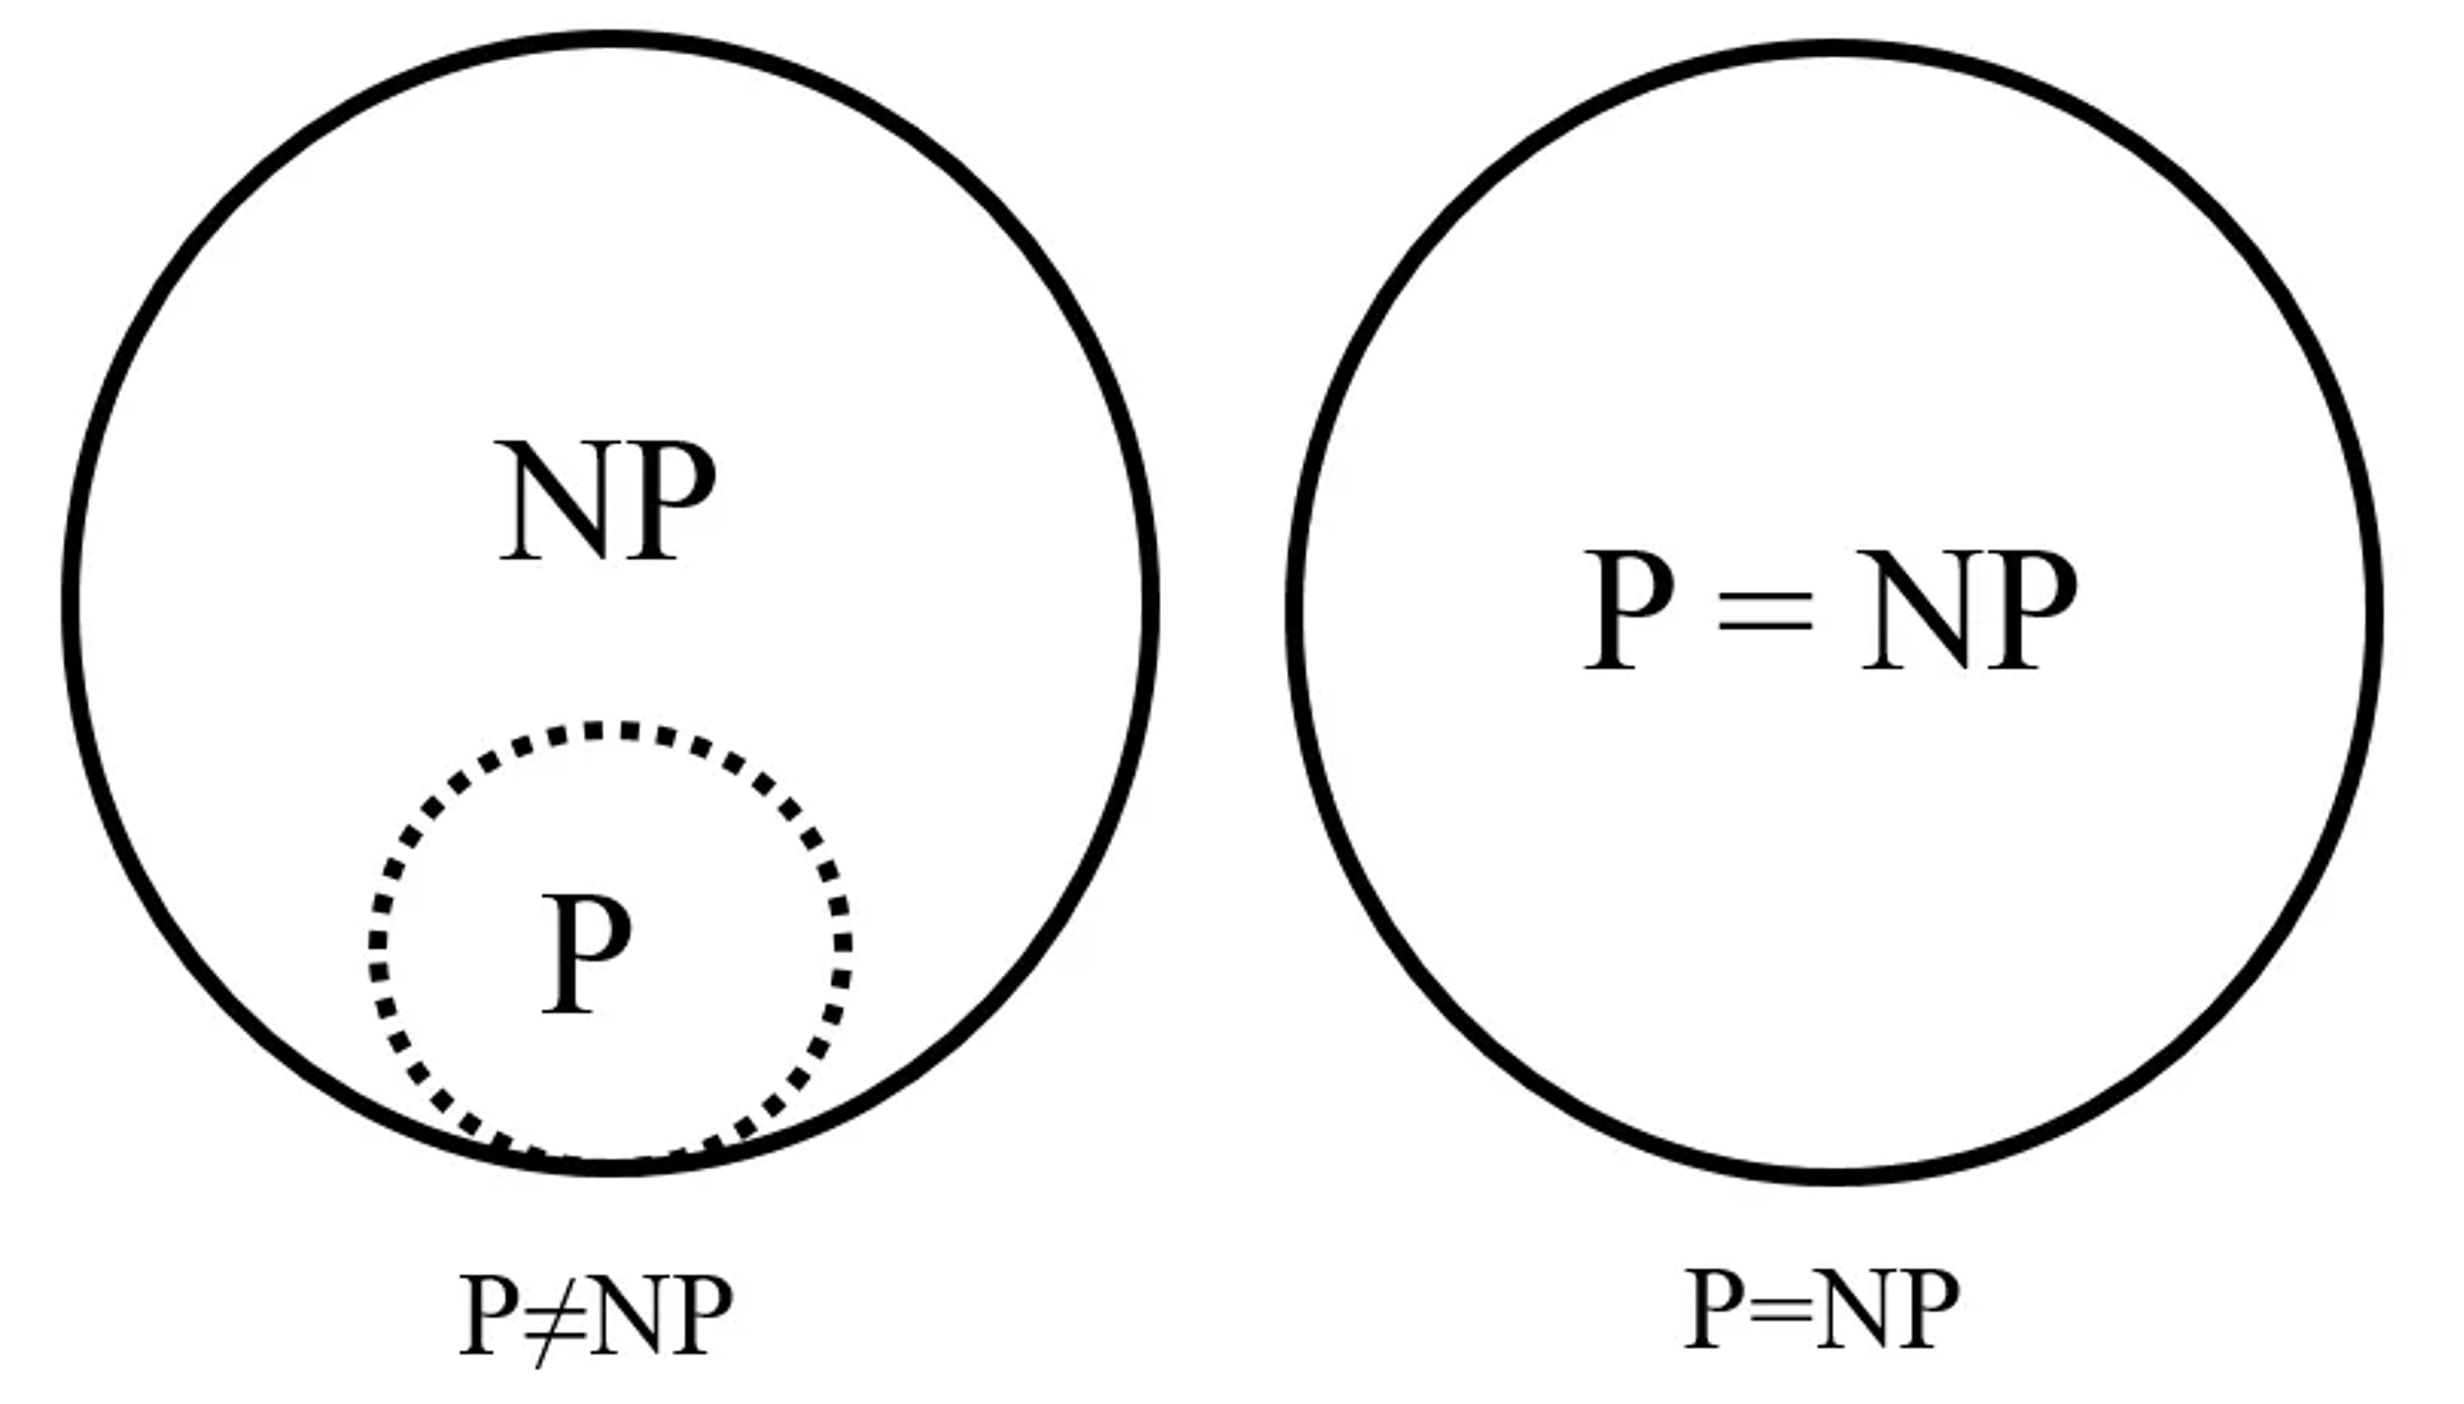
\includegraphics[scale=0.2]{PNP.jpg}
\caption{P and NP sets \cite{PNPsets}}
\end{figure}

\end{minipage}




\begin{itemize}
\item reduction explained
\end{itemize}

\begin{CountingDefinition}[Reduction]{def:validLabelPlacement}
Problem $A$ is at least as hard as problem $B$ if $B$ reduces to $A$.
\end{CountingDefinition}




\color{red} TODO \\
\color{black}
\color{violet} Questions:
\color{black}








%-------------------------------------------------------------

\subsection*{Reduction HAMILTONIAN PATH to SATISFIABLE}
\begin{itemize}
\item instance: Graph $G$ \\
question: Is there a path in $G$ that visits each node one?
\item $\log$ space reduction from HP to S
\item demonstrates HP not significantly harder that SAT
\item write a logical formular that only becomes true when it is HP
\item 4, 3, 1, 2 as path \\
$x_{1,4} = T, x_{2,3} = T,x_{3,1} = T,x_{4,2} = T,$
\item slide is not quite correct
\item $(not x_{1,1} or not x_{2,1}) and (not x_{1,1} or not x_{3,1}) \\ and (not x_{1,1} or not x_{4,1}) and (not x_{2,1} or not x_{3,1}) \\ and (not x_{2,1} or not x_{4,1}) and (not x_{3,1} or not x_{4,1}) and ...$ \\
first index: step, second: node
\end{itemize}

\color{red} TODO \\
\color{black}
\color{violet} Questions:
\color{black}







%-------------------------------------------------------------

\subsection*{Boolean Circuits}


\color{red} TODO \\
\color{black}
\color{violet} Questions:
\color{black}








%-------------------------------------------------------------

\subsection*{Reduction REACHABILITY PATH to CIRCUIT VALUE}

\color{red} TODO \\
\color{black}
\color{violet} Questions:
\color{black}







%-------------------------------------------------------------

\subsection*{Further examples}

\color{red} TODO \\
\color{black}
\color{violet} Questions:
\color{black}







%-------------------------------------------------------------

\subsection*{Closedness under Composition}


\color{red} TODO \\
\color{black}
\color{violet} Questions:
\color{black}





\newpage

\printbibliography




\end{document}